\section{Reconocimiento facial invariante a la edad}

\subsection{Objetivos}
\begin{frame}{Objetivos}

	\begin{itemize}
		\item Resolver una tarea de \textbf{reconocimiento facial invariante a cambios en la edad}, por sus siglas en inglés, \textit{AIFR}.
	\end{itemize}

	\begin{itemize}
		\item Estudiar dos \textbf{variantes \textit{online}} en la función de pérdida \textit{Triplet Loss}.
	\end{itemize}

\end{frame}

\subsection{Tarea a resolver}

\begin{frame}{\textit{AIFR}}

	\begin{figure}
		\includegraphics[width=0.8\textwidth]{informatica/ejemplo_dificultad_aifr}
		\caption{Ejemplo de datos con los que trabajamos en una tarea de \textit{AIFR}. Imagen extraída de \footcite{informatica:aifr_survey}.}
		\label{img:ejemplo_dificultad_aifr}
	\end{figure}

\end{frame}

\begin{frame}{Problemas asociados a la tarea}

	\begin{figure}
		\includegraphics[height=0.4\textheight]{informatica/ejemplo_dificultad_aifr}
	\end{figure}

	\begin{itemize}
		\item Pueden ser más similares dos personas distintas de la misma edad que la misma persona en dos edades muy distantes.
		\item El envejecimiento modifica las características faciales.
		\item Trabajar con identidades nunca vistas.
		\item Escasez de conjuntos de datos para estudiar la tarea de \textit{AIFR}, que además presentan diversas dificultades.
	\end{itemize}

\end{frame}

\subsection{Enfoque}

\begin{frame}{Embedding semántico}
	\begin{columns}
		\column{0.6\linewidth}
		\centering
		\begin{figure}
			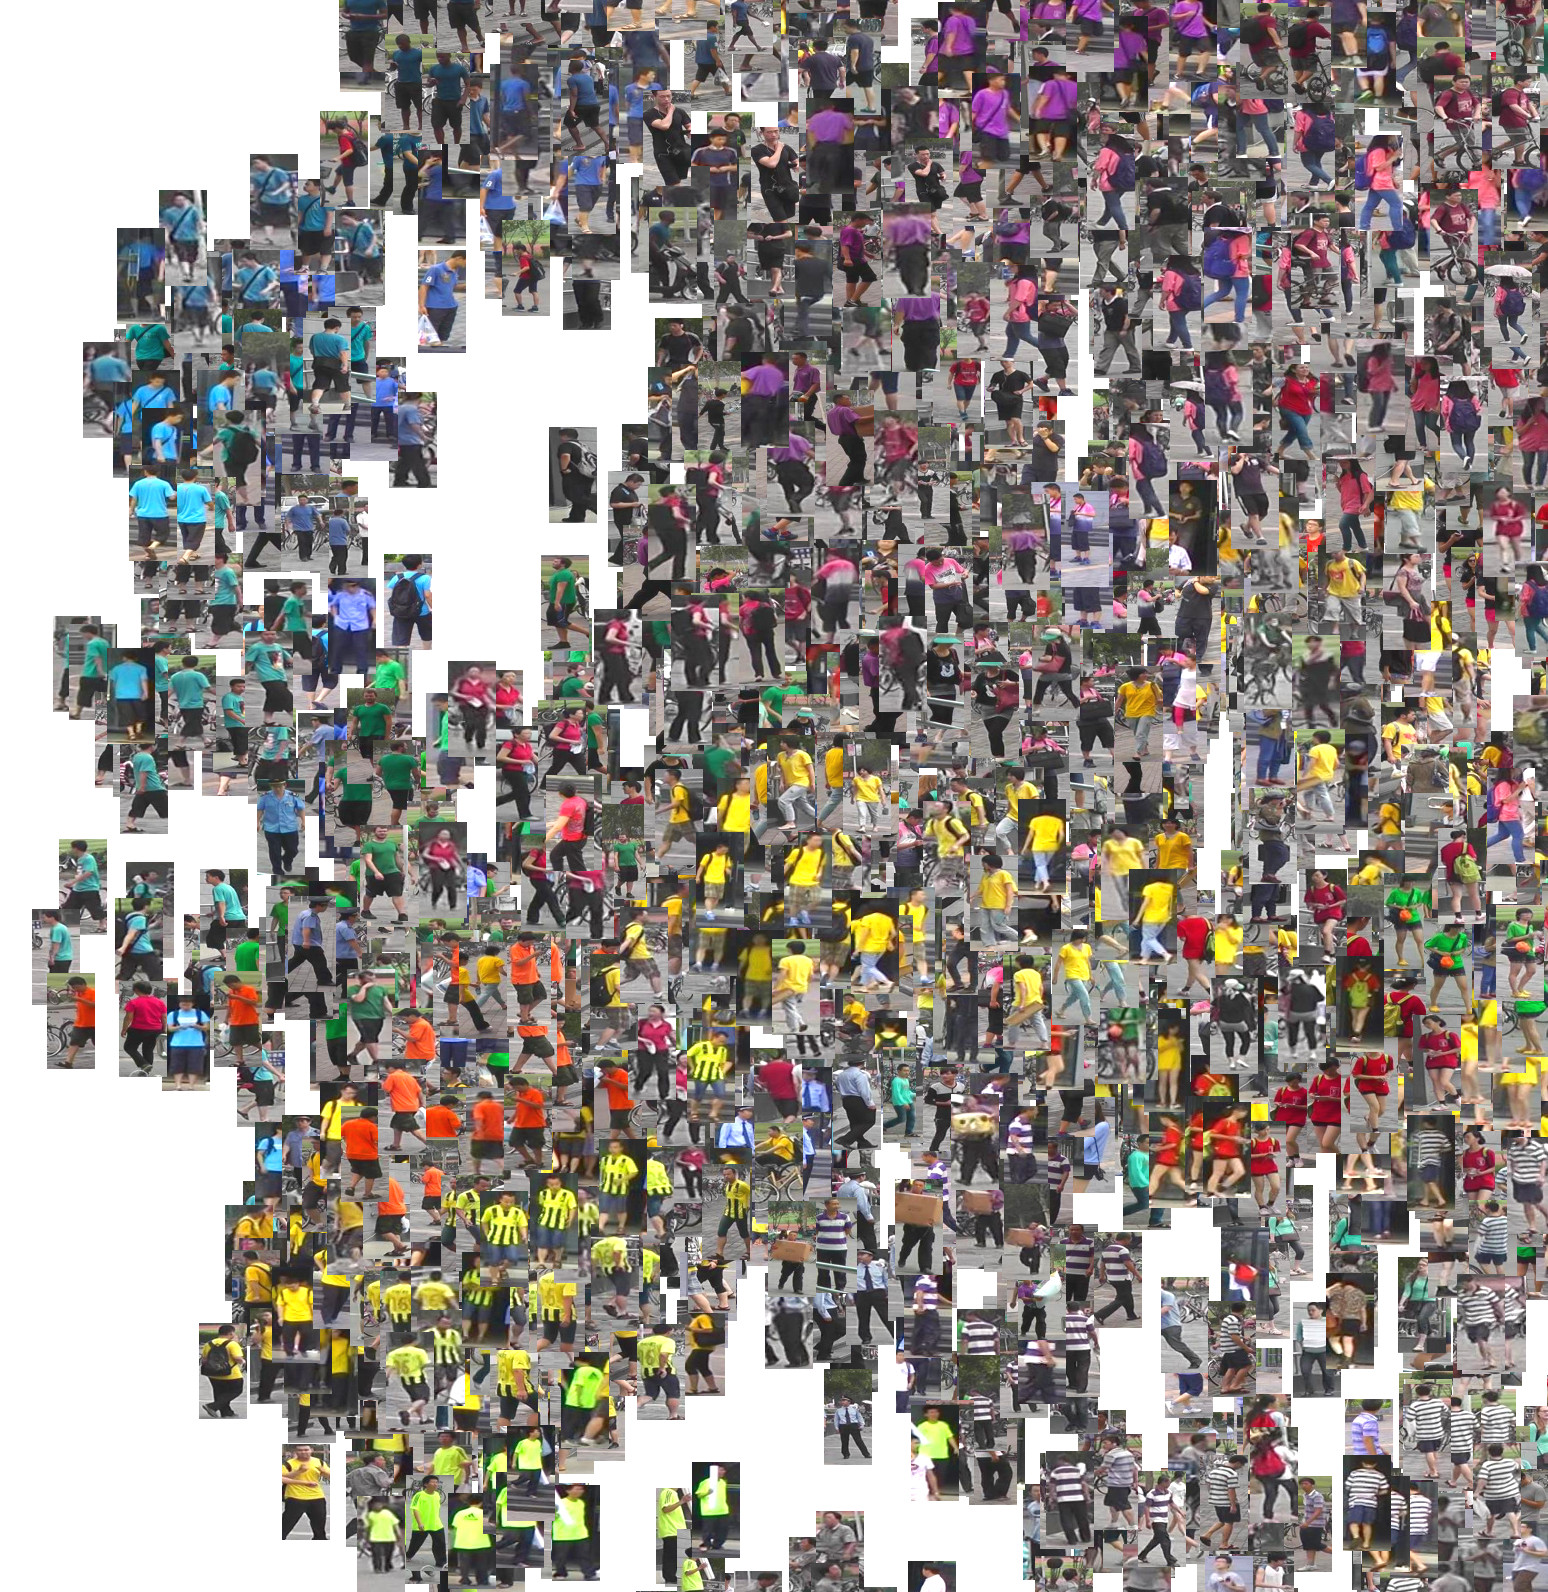
\includegraphics[width=1.0\textwidth]{informatica/embedding_paper_principal}
			\caption{Imagen extraída de \cite{informatica:principal}.}
		\end{figure}
		\column{0.5\linewidth}
		\begin{itemize}
			\item Queremos que nuestra red aprenda un \textbf{\textit{embedding} semántico}.
			\item Elementos de la misma identidad deberán estar cerca entre sí, mientras que elementos de distintas identidades deberán estar distantes.
		\end{itemize}
	\end{columns}
\end{frame}

\begin{frame}{Redes siamesas}

	\begin{figure}
		\includegraphics[width=0.9\textwidth]{informatica/siamesa_firma}
		\caption{Imagen extraída de \cite{informatica:siamesa_web_imagen}.}
		\label{img:siamesa_firma}
	\end{figure}

	\begin{itemize}
		\item Herramienta para aprender el \textit{embedding}.
		\item Se utiliza o \textit{contrastive loss} (pares) o \textit{triplet loss} (triples).
	\end{itemize}

\end{frame}

\begin{frame}{Triplet Loss}
	\begin{figure}
		\includegraphics[width=1.0\textwidth]{informatica/triplet_loss_learning}
		\caption{Imágenes extraídas de \cite{informatica:cacd_dataset}.}
	\end{figure}

	A partir de:
	\begin{equation}
		D_{A, P} \leq D_{A, N},
	\end{equation}

	llegamos a:

	\begin{equation} \label{ieq:triplet_loss_single_entry}
		\mathcal{L}_{tri}(\theta; A, P, N) := max \{D_{A, P} - D_{A, N} + \alpha, 0 \}
	\end{equation}
\end{frame}

\begin{frame}{Variantes \textit{online} sobre \textit{Triplet Loss}}

	\begin{itemize}
		\item Problema: necesitamos generar los triples de forma \textit{offline}.
		\item Solución: generar los \textit{batches} de forma \textit{online}.
		      \begin{itemize}
			      \item Usando \textit{P-K} sampling.
			      \item Aplicando las variantes \textit{Batch All} y \textit{Batch Hard} sobre estos nuevos \textit{batches}
		      \end{itemize}
	\end{itemize}

	\begin{figure}
		\includegraphics[width=0.6\textwidth]{informatica/ejemplo_grafico_pk_sampling}
		\caption{Imagen extraída de \cite{informatica:paper_image_pk_sampling}.}
	\end{figure}

\end{frame}

\begin{frame}{Variantes \textit{online}}

	Sobre el anterior \textit{P-K} sampling:

	\begin{itemize}
		\item \textbf{\textit{Batch All}}: probar todas las combinaciones ancla - positivo - negativo.
		\item \textbf{\textit{Batch Hard}}: por cada ancla, computar la pérdida con el positivo más lejano y el negativo más cercano (combinación más complicada).
	\end{itemize}

\end{frame}

\subsection{Experimentación preliminar}
\begin{frame}{Métricas más relevantes}
	\begin{itemize}
		\item \textit{Rank@k}: dada una imagen de entrada, la red devuelve las $k$ imágenes que detecta como más cercanas. Contamos como acierto si al menos una imagen corresponde a la identidad apropiada.
		\item \textit{Silhouette}: mide la calidad de los \textit{clusters} o agrupaciones obtenidas. Va desde -1 (peor valor) hasta 1 (valor perfecto).
	\end{itemize}
\end{frame}

\begin{frame}{\textit{CACD}}

	\begin{figure}
		\includegraphics[width=0.9\textwidth]{informatica/cacd_example}
		\caption{Imagen extraída de \cite{informatica:paper_cacd}}
		\label{img:cacd_imagenes_ejemplo}
	\end{figure}

\end{frame}

\begin{frame}{Resultados preliminares sobre \textit{CACD}}
	\begin{figure}
		\includegraphics[width=1.0\textwidth]{informatica/wandb/entrenamiento_principal/running_loss}
	\end{figure}
\end{frame}

\begin{frame}{Resultados preliminares sobre \textit{CACD}}
	\begin{figure}
		\includegraphics[width=1.0\textwidth]{informatica/wandb/entrenamiento_principal/intracluster_distance}
	\end{figure}
\end{frame}

\begin{frame}{Resultados preliminares sobre \textit{CACD}}
	\begin{figure}
		\includegraphics[width=1.0\textwidth]{informatica/wandb/entrenamiento_principal/intercluster_distance}
	\end{figure}

\end{frame}

\begin{frame}{Resultados preliminares sobre \textit{CACD}}
	\begin{table}
		\centering
		\begin{tabular}{|l|l|l|l|}
			\hline
			Conjunto      & \textit{Rank@1 Accuracy} & \textit{Rank@5 Accuracy} & \textit{Silhouette} \\
			\hline

			Entrenamiento & 0.07185                  & 0.15244                  & -0.41858            \\
			Test          & 0.01000                  & 0.00100                  & -0.32984            \\
			\hline
		\end{tabular}
		\caption{Valores de distintas métricas obtenidas sobre el conjunto \textit{CACD} de entrenamiento y sobre el conjunto \textit{FG-Net} de \textit{test}.}
		\label{table:resultados_sobre_fg_net}
	\end{table}

\end{frame}

\begin{frame}{Resultados preliminares sobre \textit{MNIST}}

	\begin{table}
		\centering
		\begin{tabular}{|l|l|l|l|}
			\hline
			Conjunto      & \textit{Rank@1 Accuracy} & \textit{Rank@5 Accuracy} & \textit{Silhouette} \\
			\hline

			Entrenamiento & 0.0937                   & 0.453                    & 0.000               \\
			Test          & 0.085                    & 0.414                    & 0.000               \\


			\hline
		\end{tabular}
		\caption{Métricas de evaluación obtenidas tras entrenar el modelo sobre \textit{MNIST}.}
		\label{table:resultados_mnist_mal}
	\end{table}

	En la experimentación realizada por \cite{informatica:adambielski_github} observamos los mismos problemas que estamos exponiendo.

\end{frame}

\subsection{Solución original}
\begin{frame}{Raíz del problema y nuestra propuesta de solución}
	\begin{itemize}
		\item La red aprende a transformar todas las entradas a un vector no nulo del \textit{embedding}.
		\item En esta situación tenemos que:
	\end{itemize}

	\begin{equation} \label{eq:justificacion_relu}
		\begin{split}
			\mathcal{L}(a, p, n) &= ReLU(d(a, p) - d(a, n) + \alpha) \\
			&= ReLU(d(\nv{v_0}, \nv{v_0}) - d(\nv{v_0}, \nv{v_0}) + \alpha) \\
			&= ReLU(0 - 0 + \alpha) = ReLU(\alpha) = \alpha.
		\end{split}
	\end{equation}

	\begin{itemize}
		\item Penalizar las distancias negativas pequeñas dividiendo por su media en el término ancla - positivo.
	\end{itemize}
	\begin{equation}
		\mathcal{L}(a, p, n) = \widehat{ReLU}((\widehat{d}(a, p) - \widehat{d}(a, n)) / mean(d(a, n)) + \alpha)
	\end{equation}

\end{frame}

\subsection{Validación experimental de nuestra solución}
\begin{frame}{Resultados en \textit{MNIST} con nuestra solución}

	\begin{figure}
		\includegraphics[width=0.8\linewidth]{informatica/wandb/mnist_corregido/batch_hard_running_loss.png}
	\end{figure}
\end{frame}

\begin{frame}{Resultados en \textit{MNIST} con nuestra solución}

	\begin{figure}
		\includegraphics[width=0.8\linewidth]{informatica/wandb/mnist_corregido/batch_hard_intracluster.png}
	\end{figure}

\end{frame}

\begin{frame}{Resultados en \textit{MNIST} con nuestra solución}


	\begin{figure}
		\includegraphics[width=0.8\linewidth]{informatica/wandb/mnist_corregido/batch_hard_interclusater.png}
	\end{figure}


\end{frame}

\begin{frame}{Mejora de los resultados en \textit{MNIST}}


	\begin{table}
		\centering
		\begin{tabular}{|l|l|l|l|l|}
			\hline
			Métrica                  & Conjunto      & Antes  & Después & Mejora   \\
			\hline
			\textit{Rank@1 Accuracy} & Entrenamiento & 0.0937 & 0.997   & 10.64    \\
			\textit{Rank@1 Accuracy} & Test          & 0.085  & 0.992   & 11.67    \\
			\textit{Rank@5 Accuracy} & Entrenamiento & 0.453  & 0.997   & 2.20     \\
			\textit{Rank@5 Accuracy} & Test          & 0.414  & 0.991   & 2.39     \\
			\textit{Silhouette}      & Entrenamiento & 0.000  & 0.953   & $\infty$ \\
			\textit{Silhouette}      & Test          & 0.000  & 0.922   & $\infty$ \\
			\hline
		\end{tabular}
		\label{table:comparaciones_mnist_resultados}
	\end{table}
\end{frame}

\begin{frame}{Mejora de los resultados en \textit{CACD}}

	\begin{table}
		\centering
		\begin{tabular}{|l|l|l|l|l|}
			\hline
			Métrica                  & Conjunto      & Antes   & Después & Mejora \\
			\hline
			\textit{Rank@1 Accuracy} & Entrenamiento & 0.0092  & 0.2676  & 29.09  \\
			\textit{Rank@1 Accuracy} & Test          & 0.0312  & 0.3732  & 11.96  \\
			\textit{Rank@5 Accuracy} & Entrenamiento & 0.0136  & 0.4639  & 34.11  \\
			\textit{Rank@5 Accuracy} & Test          & 0.0781  & 0.6152  & 7.88   \\
			\textit{Silhouette}      & Entrenamiento & -0.1366 & -0.1648 & -0.02  \\
			\textit{Silhouette}      & Test          & -0.1596 & -0.1832 & -0.023 \\
			\hline
		\end{tabular}
		\label{table:comparaciones_cacd_resultados}
	\end{table}


\end{frame}

\subsection{Conclusiones}
\begin{frame}{Conclusiones}

	\begin{itemize}
		\item Hemos identificado un problema de diseño en las variantes \textit{online} de \textit{Triplet Loss}.
		\item Hemos propuesto una solución original y validado experimentalmente su gran eficacia.
		\item Obtenemos buenos resultados en la tarea de \textit{AIFR}.
		\item Desarrollo en abierto de toda la base de código en nuestro repositorio de \textit{Github} \cite{informatica:repogithub}.
	\end{itemize}

\end{frame}
